\newpage
{\bfseries МРНТИ 31.17.15}

{\bfseries КОНЦЕНТРИРОВАНИЕ И ИССЛЕДОВАНИЕ ПРОДУКТОВ УГЛИСТЫХ СЛАНЦЕВ
МЕСТОРОЖДЕНИЯ БАЛА-САУСКАНДЫК}

{\bfseries \textsuperscript{1,2}С.В. Нечипуренко, \textsuperscript{2}Р.К.
Канаев, \textsuperscript{1,2}С.А.Ефремов, \textsuperscript{3}А.А.
Кузнецов, \textsuperscript{1,2}Г.А.Мун,}

\textsuperscript{1}РОО «Национальная Инженерная Академия Республики
Казахстан», Алматы, Казахстан,

\textsuperscript{2}НАО «Казахский национальный университет имени
аль-Фараби», Алматы, Казахстан,

\textsuperscript{3}ТОО «Фирма Балауса», Алматы, Казахстан

Корреспондент-автор: nechipurenkos@mail.ru

Рассмотрены особенности флотирующей способности по углероду
углерод-минерального материала. В качестве объекта исследований
выступают отходы переработки полиметаллического рудника Бала-Саускандык,
предметом исследований является углистый кек, отход после автоклавного
выщелачивания ванадиевой руды. Изучен химический анализ кека, в основу
состава которого входит углерод, диоксид кремния, соединения щелочных и
щелочноземельных металлов, а также соединения железа и алюминия.
Представленные в статье исследования показали, что для работы по
флотационному обогащению углерод-минерального материала, учитывая его
исходный рН-3, адсорбционные и электрокинетические характеристики, в
качестве реагентов флотации рекомендуется использовать реагенты с
преобладанием в основном терпеновых спиртов. Для возможности раскрытия
углерод-минерального материала для флотационного обогащения и
дальнейшего внедрения в производственный процесс проведены исследования
и расчеты определения рабочего индекса измельчаемости по методике Бонда
в шаровой мельнице с производительностью 2,72 кг/час и удельным расходом
энергии 2,62 кВт•ч/т. Исходя из результатов фракционного анализа
измельченного кека определена средняя плотность пульпы р=2,8÷3,3 или в
соотношении Т:Ж = 300÷350 г/л. В качестве реагентов для пенной флотации
опробованы синтетические ацетат 3-амилтетрагидропиран-4-ол и ксантогенат
1-метил-3-карбэтокси-1,2,5,6-тетрагидропиридин-4-ол и коммерческий
реагент-собиратель Flotol B. В качестве вспенивателя керосин
осветленный. Установлено, что оптимальным является совместное
использование керосина и «Flotol B», при этом в процессе обогащения в
одну стадию без дополнительной перечистки содержание углерода в
концентрате увеличилось до 40,0 ± 2 \%.

Получены углеродные концентраты, стабильные по химическому составу.
Учитывая гибкую схему ведения процесса обогащения возможно варьировать
содержание углерода и минеральной составляющей в концентратах, что
является важным экономическим и технологическим фактором при расчете
химико-технологических процессов. Полученные углеродные концентраты
могут быть использованы в технологических процессах производства
сорбентов, композиционных материалов и эластомеров, в качестве
альтернативных товарных материалов на основе аморфного углерода.

{\bfseries Ключевые слова:} месторождение Бала-Саускандык, отходы,
физико-химические исследования, углистый кек, флотация, флотореагент,
углерод, концентрат.

{\bfseries CONCENTRATION AND RESEARCH OF PRODUCTS OF CARBONACEOUS SHALES OF
THE BALA-SAUSKANDYK DEPOSIT}

~

{\bfseries \textsuperscript{1,2} S.V.Nechipurenko, \textsuperscript{2}R.K.
Kanaev, \textsuperscript{1,2}S.A.Yefremov,
\textsuperscript{3}A.A.Kuznetsov, \textsuperscript{1,2}G.A. Mun}

\textsuperscript{1}RPA «National Academy of Engineering of the Republic
of Kazakhstan», Almaty, Kazakhstan,

\textsuperscript{2}NJSC «al-Farabi Kazakh National University», Almaty,
Kazakhstan,

\textsuperscript{3}LLP «The Balausa company», Almaty, Kazakhstan,

e-mail:~nechipurenkos@mail.ru

~

The features of the carbon flotation capacity of a carbon-mineral
material are considered. The object of research is waste from the
processing of the polymetallic mine Bala-Sauskandyk, the subject of
research is carbonaceous cake, waste after autoclave leaching of
vanadium ore. The chemical analysis of the cake, which is based on
carbon, silicon dioxide, compounds of alkaline and alkaline earth
metals, as well as compounds of iron and aluminum, has been studied. The
research presented in the article showed that for flotation enrichment
of carbon-mineral material, taking into account its initial pH 3,
adsorption and electrokinetic characteristics, it is recommended to use
reagents with a predominance of mainly terpene alcohols as flotation
reagents. To enable the disclosure of carbon-mineral material for
flotation enrichment and further introduction into the production
process, studies and calculations were carried out to determine the
working index of shreddability using the Bond method in a ball mill with
a capacity of 2.72 kg/hour and a specific energy consumption of 2.62
kWh/t. Based on the results of fractional analysis of the crushed cake,
the average pulp density p =2.8÷3.3 or in the ratio S:L = 300÷350 g/l
was determined. Synthetic 3-amyltetrahydropyran-4-ol acetate and
1-methyl-3-carbethoxy-1,2,5,6-tetrahydropyridine-4-ol xanthogenate and
commercial collector reagent Flotol B were tested as reagents for foam
flotation. Clarified kerosene is used as a foamer. It was found that the
optimal use is the combined use of kerosene and Flotol B, while in the
process of enrichment in one stage without additional purification, the
carbon content in the concentrate increased to 40.0 ± 2\%.

Carbon concentrates stable in chemical composition were obtained. Given
the flexible scheme of the enrichment process, it is possible to vary
the content of carbon and mineral components in concentrates, which is
an important economic and technological factor in the calculation of
chemical and technological processes. The resulting carbon concentrates
can be used in technological processes for the production of sorbents,
composite materials and elastomers, as alternative commercial materials
based on amorphous carbon.

{\bfseries Keywords:} Bala-Sauskandyk deposit, waste, physico-chemical
studies, carbon cake, flotation, flotation reagents, carbon,
concentrate.

{\bfseries БАЛА-САУСКАНДЫҚ КЕН ОРНЫНЫҢ КӨМІРТЕКТІ ТАҚТАТАС ӨНІМДЕРІН
ШОҒЫРЛАНДЫРУ ЖӘНЕ ЗЕРТТЕУ}

~

{\bfseries \textsuperscript{1,2}С.В. Нечипуренко, \textsuperscript{2}Р.К.
Канаев, \textsuperscript{1,2}С.А.Ефремов,
\textsuperscript{3}А.А.Кузнецов, \textsuperscript{1,2}Г.А.Мун}

\textsuperscript{1}«Қазақстан Республикасының Ұлттық Инженерлік
Академиясы» РҚБ, Алматы, Қазақстан,

\textsuperscript{2}«әл-Фараби атындағы Қазақ ұлттық университеті» КЕАҚ,
Алматы, Қазақстан,

\textsuperscript{3}«Фирма Балауса» ЖШС, Алматы, Қазақстан,

e-mail:~nechipurenkos@mail.ru

~

Көміртек-минералды материалдың көміртегі бойынша флотация қабілетінің
ерекшеліктері қарастырылды. Зерттеу нысаны ретінде Бала-Саускандық
полиметалл кенішінің қайта өңдеу қалдықтары, зерттеу пәні көміртекті
кек, ванадий кенін автоклавты шаймалаудан кейінгі қалдықтар болып
табылады. Кектің химиялық талдауы зерттелді, оның құрамына көміртегі,
кремний диоксиді, сілтілік және жер сілтілік металдардың қосылыстары,
сондай-ақ темір мен алюминий қосылыстары кіреді. Мақалада келтірілген
зерттеулер көміртегі-минералды материалды флотациялық байыту бойынша
жұмыс істеу үшін оның бастапқы pН 3, адсорбциялық және
электрокинетикалық сипаттамаларын ескере отырып, флотация реагенттері
ретінде негізінен терпен спирттері басым реагенттерді қолдану
ұсынылатынын көрсетті. Флотациялық байыту және өндірістік процеске одан
әрі енгізу үшін көміртек-минералды материалды ашу мүмкіндігі үшін
өнімділігі 2,72 кг/сағ және энергияның меншікті шығыны 2,62 кВт•сағ/т
шар диірменінде Бонд әдістемесі бойынша ұсақталудың жұмыс индексін
анықтау бойынша зерттеулер мен есептеулер жүргізілді. Ұсақталған кекті
фракциялық талдау нәтижелеріне сүйене отырып, пульпаның орташа тығыздығы
анықталды р=2,8÷3,3 немесе Қ:С қатынасында = 300÷350 г/л. Көбік
флотациясы үшін реагенттер ретінде синтетикалық ацетат
3-амилтетрагидропиран-4-ол және ксантогенат
1-метил-3-карбэтокси-1,2,5,6-тетрагидропиридин-4-ол және Flotol B
коммерциялық реагент-жинаушы сыналды. Көбіктендіргіш ретінде
жеңілдетілген керосин қолданылды. Керосин мен "Flotol B" бірге қоладану
оңтайлы екендігі анықталды, бұл ретте байыту процесінде концентраттағы
көміртегі мөлшері қосымша тазартусыз бір сатыда 40,0 ± 2 \% дейін өсті.

Химиялық құрамы бойынша тұрақты көміртекті концентраттар алынды. Байыту
процесін жүргізудің икемді сызбанұсқасын ескере отырып, химиялық және
технологиялық процестерді есептеу кезінде маңызды экономикалық және
технологиялық фактор болып табылатын концентраттардағы көміртегі мен
минералды компоненттердің құрамын өзгертуге болады. Алынған көміртегі
концентраттарын сорбенттерді, композициялық материалдарды және
эластомерлерді өндірудің технологиялық процестерінде, аморфты көміртегі
негізіндегі балама тауарлық материалдар ретінде пайдалануға болады.

{\bfseries Түйінді сөздер:} Бала-Саускандық кен орны, қалдықтар,
физика-химиялық зерттеулер, көміртекті кек, флотация, флотореагенттер,
көміртек, концентрат.

{\bfseries Введение.} Актуальной задачей современных производств является
комплексное использование природных ресурсов и создание безотходных
технологий. В этой связи в последнее десятилетия существенное изменение
претерпело отношение к отходам. С точки зрения рационального
природопользования промышленные отходы являются вторичными материальными
ресурсами. Широко известно большое значение углеродных материалов (сажи,
активированного угля и др.) для различных отраслей промышленности.
Учитывая сложный минералогический и химический составы
углеродсодержащего сырья, залегающего в рудном теле и в отвалах
промышленных предприятий, разработка безотходной технологии переработки,
получение новых многофункциональных материалов, становится актуальной
проблемой, имеющей как научное, так и практическое значение {[}1,2{]}.

В статье представлены материалы по обогащению углистого кека, отхода
после автоклавного выщелачивания ванадиевой руды месторождения
Бала-Саускандык. Изучены физико-химические характеристики углистого кека
и продуктов обогащения.

{\bfseries Материалы и методы.} В качестве источника для получения ряда
углеродсодержащих материалов многоцелевого использования, могут служить
углистые сланцы («кеки») -- отходы переработки полиметаллического
рудника Бала-Саускандык. Месторождение Бала-Саускандык разрабатываемое
компанией Ferro-Alloy Resources Group, представляет собой крупное
ванадиевое месторождение, расположенное в Кызылординской области в Южном
Казахстане {[}3{]}.

Предметом исследований явились углистые «кеки», отходы после
автоклавного выщелачивания ванадиевой руды.

Основной технологический процесс производства предприятия представляет
собой низкотемпературный натрирующий обжиг с последующим выщелачиванием,
сорбцией, десорбцией и осаждением солей ванадия и молибдена. Основа
материала составляет глинозем, и углеродная составляющая остается в
твердой фазе -- «кек». Данный кек после фильтрации отправляется как
низкосортный материал на строительные нужды или направляется в отвалы
{[}4{]}.

Проведенный химический анализ кека показывает неоднородность его
состава. Анализ проводили рентгеноспектральным методом в ТОО ЦЛ
«ГеоАналитика», категория точности анализа -- III, по СТ РК 1354-2005
инструкция НСАМ №313-РС. Определение содержания общего углерода
проводили при температуре 850-900 ℃ в муфельной печи в воздушной
атмосфере, в таблице 1 отмечено как п.п.п. -- потери после прокаливания.
Выбор данного метода определения углерода обусловлен тем, что исходная
ванадиевая руда подвергается агрессивному воздействию и, следовательно,
в углистом кеке после обогащения отсутствует органический углерод.

Результаты исследований говорят о том, что данный кек -- это сложная
система, в состав которой входят уг­лерод, диоксид кремния, соединения
щелочных и щелочноземельных ме­тал­лов, а также соединения железа,
алюминия, таблица 1. Для всех исследований в работе углистый кек был
предварительно просушен при температуре 105±2℃ для стабилизации по
влажности до показания не более 1,0 \%.

Таблица 1 - Химический состав «кека» и продуктов обогащения

\begin{longtable}[]{@{}
  >{\raggedright\arraybackslash}p{(\columnwidth - 16\tabcolsep) * \real{0.1819}}
  >{\raggedright\arraybackslash}p{(\columnwidth - 16\tabcolsep) * \real{0.1062}}
  >{\raggedright\arraybackslash}p{(\columnwidth - 16\tabcolsep) * \real{0.1061}}
  >{\raggedright\arraybackslash}p{(\columnwidth - 16\tabcolsep) * \real{0.0909}}
  >{\raggedright\arraybackslash}p{(\columnwidth - 16\tabcolsep) * \real{0.0910}}
  >{\raggedright\arraybackslash}p{(\columnwidth - 16\tabcolsep) * \real{0.0909}}
  >{\raggedright\arraybackslash}p{(\columnwidth - 16\tabcolsep) * \real{0.0859}}
  >{\raggedright\arraybackslash}p{(\columnwidth - 16\tabcolsep) * \real{0.0900}}
  >{\raggedright\arraybackslash}p{(\columnwidth - 16\tabcolsep) * \real{0.1571}}@{}}
\toprule\noalign{}
\multirow{2}{*}{\begin{minipage}[b]{\linewidth}\raggedright
№ пробы
\end{minipage}} & \multicolumn{8}{l@{}}{%
\begin{minipage}[b]{\linewidth}\raggedright
Содержание, \%~
\end{minipage}} \\
& \begin{minipage}[b]{\linewidth}\raggedright
Fe\textsubscript{2}O\textsubscript{3}
\end{minipage} & \begin{minipage}[b]{\linewidth}\raggedright
Al\textsubscript{2}O\textsubscript{3}
\end{minipage} & \begin{minipage}[b]{\linewidth}\raggedright
SiO\textsubscript{2}
\end{minipage} & \begin{minipage}[b]{\linewidth}\raggedright
TiO\textsubscript{2}
\end{minipage} & \begin{minipage}[b]{\linewidth}\raggedright
MnO
\end{minipage} & \begin{minipage}[b]{\linewidth}\raggedright
V\textsubscript{2}O\textsubscript{5}
\end{minipage} & \begin{minipage}[b]{\linewidth}\raggedright
п.п.п.
\end{minipage} & \begin{minipage}[b]{\linewidth}\raggedright
Сумма
\end{minipage} \\
\midrule\noalign{}
\endhead
\bottomrule\noalign{}
\endlastfoot
Пр № 1 исх & 9,20 & 2,62 & 75,12 & 0,44 & \textless0,10 & 0,53 & 14,19 &
100,00 \\
Пр № 1 конц. & 2,45 & 7,74 & 48,18 & 0,37 & \textless0,10 & 0,44 & 39,53
& 100,00 \\
Пр № 1 хвост & 10,73 & 2,00 & 82,80 & 0,17 & \textless0,10 & 0,42 & 7,43
& 100,00 \\
\end{longtable}

Проведены исследования на понимание каким образом флотореагенты и
электролиты (активатор или депрессор) адсорбируются на поверхности
углерод-минерального материала в зависимости от рН среды. В качестве
наиболее информативного примера, было рассмотрено, как закрепляется
бутиловый ксантогенат (БКс) на поверхности углерод-минерального
материала и флотационного концентрата. Проведены исследования факторов,
влияющих на адсорбцию ионов ПАВ на границе раздела фаз, с учетом
взаимодействия в области двойного электрического слоя.

Проведены работы по определению рабочего индекса измельчаемости
углерод-минерального кека по методике Бонда. Исследования проводились на
представительной пробе углерод-минерального кека, класс крупности минус
2,5 мм в шаровой мельнице типа МЛ-40 объемом 9,0 дм\textsuperscript{3},
общий вес шаровой загрузки составлял 9,46 кг, диаметры шаров от 16 до 40
мм. Разделение измельченного продукта проводилось на сите с ячейками
0,074 × 0,074 мм. Далее готовый продукт сушился, взвешивался и по
разности с первоначальной навеской определялся выход остатка на сите
+0,074мм. После этого к нему добавлялась исходный материал по массе до
принятой навески и вода по заданному для данного опыта отношению Т : Ж.
Приготовленное таким способом питание мельницы вводилось в последующий
цикл измельчения. Продолжительность измельчения измерялась количеством
оборотов вращения барабана мельницы. Частота вращения барабана 73
мин\textsuperscript{-1}. Испытание в замкнутом цикле считается
установившимся, если обеспечивается выход готового продукта по массе
близкий к тому, который необходим для 250-270\% циркулирующей нагрузки.

Проведен фракционный и ситовой анализ. К фракционному анализу относится
метод разделения отдельных групп минеральных ча­стиц, отличающихся по
плотности. Фракцион­ный состав продуктов отсадки дает наиболее
объективную и полную информацию о точности разделения исходного
мате­риала по плотности. Проведение фракционного анализа проводили в
соответствии с {[}5{]}. Для расслоения исследуемого материала размером
зерен менее 0,63 мм применяли органические жидкости плотностью от 1300
до 2600 кг/м\textsuperscript{3}, раствор хлористого цинка плотностью от
1100 до 2000 кг/м\textsuperscript{3} и органические жидкости плотностью
от 2000 до 2600 кг/м\textsuperscript{3}.

Проведено флотационное обогащение углистого кека по углероду. Как
известно, основными свойствами флотационной пульпы, влияющими на процесс
флотации, являются ее плотность, температура и концентрация водородных
ионов. Плотность пульпы измеряется отношением массы твердого к массе
воды Т:Ж или р = Ж:Т; содержанием твердого в 1 л пульпы (г/л) или
содержанием твердого в процентах. С увеличением плотности пульпы
повышается производительность флотационной установки, снижаются расходы
реагентов на единицу объема пульпы, электроэнергии и воды. Однако при
чрезмерном увеличении плотности пульпы понижается аэрация и ухудшается
флотация крупных частиц вследствие их отрыва от пузырьков воздуха при
столкновении с соседними частицами. При этом происходит интенсивная
флотация тонких частиц породы, загрязняющих концентрат. Потери
углеродной части с отходами увеличиваются. Процесс флотационного
обогащения проводился на лабораторной флотационной машине ФМУ-М2, объем
камеры 3,0 дм/м\textsuperscript{3} {[}6-8{]}.

{\bfseries Результаты и обсуждения.} \emph{1. Определение флотирующей
способности и адсорбционные свойства углистого кека.} Необходимым
требованием, предъявляемым к сырьевым материалам, используемым в
технологическом переделе, является постоянство химического и
гранулометрического составов. Учитывая, что химический состав кека
непостоянен, нами были проведены работы по стабилизации его состава
{[}9{]} методом флотационного обогащения.

Наиболее важными показателями флотирующей способности являются ---
смачиваемость поверхности твердой фазы и адсорбционные свойства
материала при взаимодействии с флотационными реагентами.

На первом этапе было важно понять каким образом флотореагенты и
электролиты (активатор или депрессор) адсорбируются на поверхности
углистого кека в зависимости от рН среды. В качестве наиболее
информативного примера, было рассмотрено, как закрепляется бутиловый
ксантогенат (БКс) на поверхности кглистого кека и флотационного
концентрата. Адсорбцию БКс на границе раздела вода-воздух проводили
путем измерения поверхностного натяжения их растворов методом отрыва
пластинки Вильгельми {[}10{]}. Данные этих определений приведены на
рисунке 1. Из которых видно, что с увеличением рН среды адсорбция БКс
снижается, что может быть связано с гидрофилизацией поверхности
углистого кека гидроксил-ионами.

\begin{figure}[H]
	\centering
	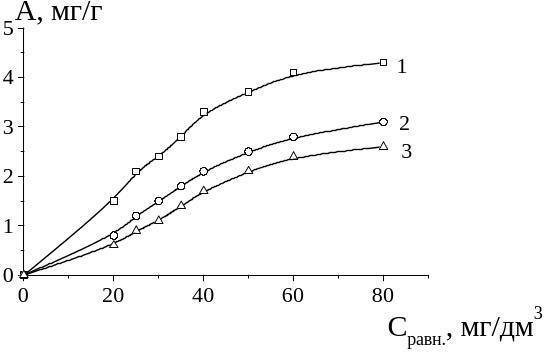
\includegraphics[width=0.8\textwidth]{assets/1033}
	\caption*{}
\end{figure}\begin{figure}[H]
	\centering
	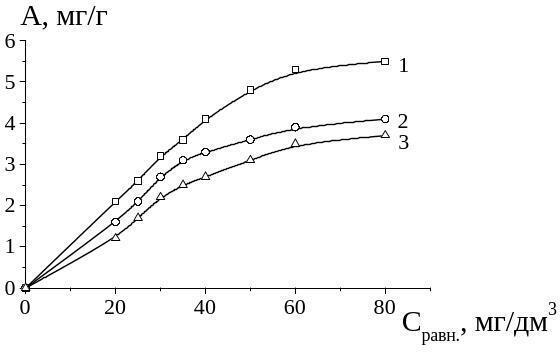
\includegraphics[width=0.8\textwidth]{assets/1034}
	\caption*{}
\end{figure}

А)1 -- рН = 3; 2 -- рН =6; 3 -- рН = 8 Б) 1 -- рН = 3; 2 -- рН =6; 3 --
рН = 8

{\bfseries Рис. 1- Зависимость адсорбции БКс на поверхности углистого кека
А и флотационного}

{\bfseries концентрата Б, при разных рН среды}

В пользу такого предположения свидетельствуют электрокинетические
данные, которые представлены на рисунке 2. Измерение
электрокинетического потенциала частиц флотируемого материала проводили
в несколько видоизмененном приборе Рабиновича и Фодиман по методу
подвижной границы раздела вода-суспензия {[}11{]}. Показано, что с
увеличением рН среды отрицательный заряд углистого кека увеличивается за
счет преимущественной адсорбции гидроксил-ионов. При увеличении
концентрации БКс отрицательный заряд поверхности также увеличивается. за
счет гидрофобных взаимодействий между углеводородными радикалами БКс и
алифатическими метиленовыми группами циклических нафтеновых фаз
углеродного материала. В результате этого полярные группы БКс будут
обращены в водную фазу, что придает материалу отрицательный
дополнительный заряд. Следует отметить, что из-за большей доступности
гидрофобных участков на поверхности обогащенного углистого кека для
молекул БКс создаются благоприятные условия для сорбции его молекул.

Хорошо известно, что одним из основных факторов, влияющих на адсорбцию
ионов ПАВ на границе раздела фаз, являются взаимодействия в области
двойного электрического слоя. Образование поверхностного заряда при
контакте твердой фазы с водным раствором характерно почти для всех
систем. Только в определенных условиях, существующих в растворе, общий
поверхностный заряд равен нулю, что соответствует точке нулевого заряда
(ТНЗ). Чтобы система в целом оставалась электронейтральной, в растворе
должно находиться одинаковое число ионов с противоположными по знаку
зарядами, эта совокупность электрических зарядов противоположных знаков,
распределенных вдоль границы, раздела двух фаз, образует двойной
электрический слой {[}12,13{]}.

\begin{figure}[H]
	\centering
	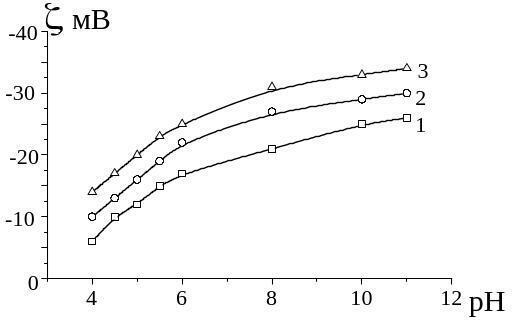
\includegraphics[width=0.8\textwidth]{assets/1035}
	\caption*{}
\end{figure}

{\bfseries Рис. 2- Зависимость электрокинетического потенциала частиц
углистого кека (углерод -19,5 \% масс.) (1); флотационного концентрата
(углерод -39,5 \% масс.) (2) и концентрата, после дополнительного
химического обогащения (углерод - 73,2 \%) (3) от рН среды}

Таким образом, проведенные исследования показали, что для работы по
флотационному обогащению углистого кека, учитывая его исходный рН-3, а
так же адсорбционные и электрокинетические характеристики в качестве
реагентов флотации использовались реагенты с преобладанием в основном
терпеновых спиртов.

\emph{2. Определение рабочего индекса измельчаемости углистого кека по
методике Бонда.}

Результаты испытаний по определению индекса измельчаемости углистого
кека приведены в таблице 2.

{\bfseries Таблица 2 -- Результаты испытаний по определению индекса
измельчаемости углистого кека}

\begin{longtable}[]{@{}
  >{\raggedright\arraybackslash}p{(\columnwidth - 8\tabcolsep) * \real{0.1924}}
  >{\raggedright\arraybackslash}p{(\columnwidth - 8\tabcolsep) * \real{0.1588}}
  >{\raggedright\arraybackslash}p{(\columnwidth - 8\tabcolsep) * \real{0.2462}}
  >{\raggedright\arraybackslash}p{(\columnwidth - 8\tabcolsep) * \real{0.1623}}
  >{\raggedright\arraybackslash}p{(\columnwidth - 8\tabcolsep) * \real{0.2402}}@{}}
\toprule\noalign{}
\begin{minipage}[b]{\linewidth}\raggedright
Циклы измельчения
\end{minipage} & \begin{minipage}[b]{\linewidth}\raggedright
Число оборотов мельницы за 1 цикл
\end{minipage} & \begin{minipage}[b]{\linewidth}\raggedright
Кол-во материала

-0,074мм, образовавшегося за циклы, г
\end{minipage} & \begin{minipage}[b]{\linewidth}\raggedright
Остаток материала на сите +0,074мм, г
\end{minipage} & \begin{minipage}[b]{\linewidth}\raggedright
Циркуляционная нагрузка,

\%
\end{minipage} \\
\midrule\noalign{}
\endhead
\bottomrule\noalign{}
\endlastfoot
1 & 145 & 230,0 & 770,0 & 335 \\
2 & 325 & 205,0 & 795,0 & 388 \\
3 & 425 & 260,0 & 740,0 & 285 \\
4 & 438 & 275,0 & 725,0 & 264 \\
\end{longtable}

После стабилизации показателей измельчения определялась
гранулометрическая характеристика готового продукта (таблица 3)
{[}14,15{]} методом ситового анализа.

{\bfseries Таблица 3 -- Гранулометрическая характеристика исходного и
измельченного кека}

\begin{longtable}[]{@{}
  >{\raggedright\arraybackslash}p{(\columnwidth - 12\tabcolsep) * \real{0.1424}}
  >{\raggedright\arraybackslash}p{(\columnwidth - 12\tabcolsep) * \real{0.1206}}
  >{\raggedright\arraybackslash}p{(\columnwidth - 12\tabcolsep) * \real{0.1524}}
  >{\raggedright\arraybackslash}p{(\columnwidth - 12\tabcolsep) * \real{0.1561}}
  >{\raggedright\arraybackslash}p{(\columnwidth - 12\tabcolsep) * \real{0.1206}}
  >{\raggedright\arraybackslash}p{(\columnwidth - 12\tabcolsep) * \real{0.1525}}
  >{\raggedright\arraybackslash}p{(\columnwidth - 12\tabcolsep) * \real{0.1554}}@{}}
\toprule\noalign{}
\multicolumn{4}{@{}l}{%
\begin{minipage}[b]{\linewidth}\raggedright
Исходный кек
\end{minipage}} & \multicolumn{3}{l@{}}{%
\begin{minipage}[b]{\linewidth}\raggedright
Измельченный кек
\end{minipage}} \\
\midrule\noalign{}
\endhead
\bottomrule\noalign{}
\endlastfoot
\multirow{2}{*}{Размер сита, мм} & \multicolumn{2}{l} & \multirow{2}{*}{суммарный выход
классов, прошедших через сито, \%} & \multicolumn{2}{l} & \multirow{2}{*}{суммарный выход
классов, прошедших через сито, \%} \\
& частный & суммарный & & частный & суммарный \\
-2,5+1,0 & 62,0 & 62,0 & 100 & 10,02 & 10,02 & 100,00 \\
-1,0+0,5 & 13,0 & 75,0 & 38,0 & 5,11 & 15,13 & 89,98 \\
-0,5+0,2 & 11,6 & 86,6 & 25,0 & 25,05 & 40,18 & 84,87 \\
-0,2+0,1 & 7,4 & 94,0 & 13,4 & 10,74 & 50,92 & 59,82 \\
-0,1+0,074 & 4,0 & 98,0 & 6,0 & 21,47 & 72,39 & 49,08 \\
0,074+0,044 & 1,8 & 99,8 & 2,0 & 14,83 & 87,22 & 27,61 \\
Итого: & 100,0 & & & 100,0 & & \\
\end{longtable}

Расход энергии, потребляемой при измельчении, определялся с помощью
трехфазного счетчика. Полезная энергия, затрачиваемая на измельчение,
определялась по разности показаний счетчика при работе мельницы под
нагрузкой и без нее при вращении пустого барабана по формуле:

\begin{figure}[H]
	\centering
	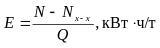
\includegraphics[width=0.8\textwidth]{assets/1036}
	\caption*{}
\end{figure}{\bfseries ,}

где Е -- удельный расход энергии, затраченной только на измельчение,
кВтч/т;

N -- мощность, потребляемая при измельчении, кВт;

N\textsubscript{х-х} -- мощность холостого хода мельницы без
измельчающей среды, кВт;

Q -- производительность мельницы по исходному питанию, т/ч.

Производительность шаровой мельницы Q рассчитывалась по времени
измельчения t (сек) и навеске кека Р (кг):

\begin{figure}[H]
	\centering
	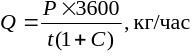
\includegraphics[width=0.8\textwidth]{assets/1037}
	\caption*{}
\end{figure}

где С -- циркулирующая нагрузка, доли единицы, в нашем случае равны
2,68.

\begin{figure}[H]
	\centering
	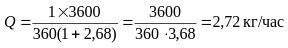
\includegraphics[width=0.8\textwidth]{assets/1038}
	\caption*{}
\end{figure}

Удельный расход энергии равен:

\begin{figure}[H]
	\centering
	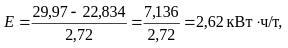
\includegraphics[width=0.8\textwidth]{assets/1039}
	\caption*{}
\end{figure}

Индекс чистой работы измельчения в шаровой мельнице по Бонду определялся
по формуле:

\begin{figure}[H]
	\centering
	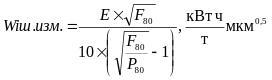
\includegraphics[width=0.8\textwidth]{assets/1040}
	\caption*{}
\end{figure}

F\textsubscript{80} и Р\textsubscript{80} -- размеры отверстий сит,
через которые соответственно проходит 80\% исходного питания и готового
продукта измельчения, мкм.

Параметры F\textsubscript{80} и Р\textsubscript{80} для исследуемого
кека определялся по кривым, представленным на рисунке 3.

\begin{figure}[H]
	\centering
	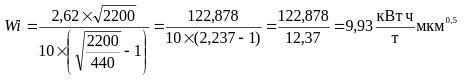
\includegraphics[width=0.8\textwidth]{assets/1041}
	\caption*{}
\end{figure}

\begin{figure}[H]
	\centering
	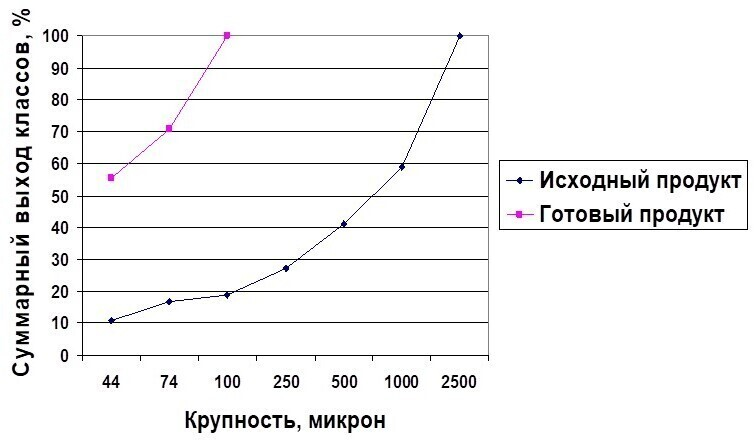
\includegraphics[width=0.8\textwidth]{assets/1042}
	\caption*{}
\end{figure}

{\bfseries Рис.3- Гранулометрическая характеристика исходного и конечного
продуктов измельчения}

Анализ полученных расчетных данных и зависимостей позволил сделать вывод
о равномерном распределении работы измельчения без необходимости
проводить многостадийное измельчение для проведения дальнейшего
флотационного обогащения.

Испытание в замкнутом цикле считается установившимся, т.к.
обеспечивается выход готового продукта по массе для 250-270\%
циркулирующей нагрузки.

\emph{3. Обогащение углистого кека пенной флотацией.}

Одним из важных параметров обогащаемого материала является фракционный
состав. Фракционный анализ кека размером зерен менее 0,63 мм проводили
методом центрифугирования. Для исследований использовались растворы
хлористого цинка плотностью от 1300 кг/м\textsuperscript{3} до 1800
кг/м\textsuperscript{3} . Результаты фракционного и ситового анализа
представлены в таблице 4 и 5.

{\bfseries Таблица 4 - Фракционный анализ углистого кека}

\begin{longtable}[]{@{}
  >{\raggedright\arraybackslash}p{(\columnwidth - 6\tabcolsep) * \real{0.2729}}
  >{\raggedright\arraybackslash}p{(\columnwidth - 6\tabcolsep) * \real{0.1513}}
  >{\raggedright\arraybackslash}p{(\columnwidth - 6\tabcolsep) * \real{0.2731}}
  >{\raggedright\arraybackslash}p{(\columnwidth - 6\tabcolsep) * \real{0.3027}}@{}}
\toprule\noalign{}
\endhead
\bottomrule\noalign{}
\endlastfoot
\multirow{2}{*}{Плотность фракций, кг/м\textsuperscript{3}} &
\multirow{2}{*}{Выход фракций,

\%} &
\multicolumn{2}{>{\raggedright\arraybackslash}p{(\columnwidth - 6\tabcolsep) * \real{0.5758} + 2\tabcolsep}@{}} \\
& & всплывшие фракции & невсплывшие фракции \\
\textless{} 1300

1300-1400

1400-1500

1500-1800

\textgreater{} 1800 & 60,5

22,6

4,9

3,1

8,9 & 60,5

83,1

88,0

91,1

100 & 100

39,5

16,9

12,0

8,9 \\
\end{longtable}

Параллельно с фракционным анализом был проведен ситовый анализ
используемого кека для флотации. Класс крупности рабочей фракции
составил − 0,63 мм.

{\bfseries Таблица 5 - Ситовой состав исходной пробы углистого кека}

\begin{longtable}[]{@{}
  >{\raggedright\arraybackslash}p{(\columnwidth - 8\tabcolsep) * \real{0.2899}}
  >{\raggedright\arraybackslash}p{(\columnwidth - 8\tabcolsep) * \real{0.1629}}
  >{\raggedright\arraybackslash}p{(\columnwidth - 8\tabcolsep) * \real{0.1776}}
  >{\raggedright\arraybackslash}p{(\columnwidth - 8\tabcolsep) * \real{0.1925}}
  >{\raggedright\arraybackslash}p{(\columnwidth - 8\tabcolsep) * \real{0.1771}}@{}}
\toprule\noalign{}
\endhead
\bottomrule\noalign{}
\endlastfoot
Фракция, мм & -0,63+0,20 & -0,20+0,074 & -0,074+0,044 & -0,044+0,00 \\
Содержание, \% масс. & 11,3 & 23,7 & 46,1 & 18,9 \\
\end{longtable}

При флотационном обогащении углистого кека средняя плотность пульпы
принималась как р=2,8÷3,3 или Т:Ж = 300÷350 г/л. Такое соотношение Т:Ж
было определено как оптимальное. Учитывая адсорбционные и
электрокинетические характеристики исследуемого материала, описанных
выше, в качестве реагентов для пенной флотации были опробованы
синтетические ацетат 3-амилтетрагидропиран-4-ол и ксантогенат
1-метил-3-карбэтокси-1,2,5,6-тетрагидропиридин-4-ол, синтезированные в
НАО «КазНУ им. аль-Фараби», а также коммерческий реагент-собиратель
Flotol B. В качестве собирателя керосин осветленный. Дозирование
флотационных реагентов велось дробно, через дозаторы. Режимные параметры
ведения процесса флотации экспериментально определенные, как
оптимальные, представлены в таблице 6.

{\bfseries Таблица 6 -- Режимные параметры технологического процесса
флотации, пересчитанные на 1 тонну углистого кека на флотацию}

\begin{longtable}[]{@{}
  >{\raggedright\arraybackslash}p{(\columnwidth - 4\tabcolsep) * \real{0.6434}}
  >{\raggedright\arraybackslash}p{(\columnwidth - 4\tabcolsep) * \real{0.1753}}
  >{\raggedright\arraybackslash}p{(\columnwidth - 4\tabcolsep) * \real{0.1814}}@{}}
\toprule\noalign{}
\endhead
\bottomrule\noalign{}
\endlastfoot
Наименование параметра & Ед. изм. & Значение \\
Расход вспенивателя на 1 тонну руды & г & 320 \\
Расход собирателя на 1 тонну руды & г & 280 \\
Содержание класса -0,074 мм в питании флотации & \% & 65 \\
Плотность питания основной флотации & \% тв & 30 \\
\end{longtable}

Основной характеристикой качества флотореагентов является устойчивость
пены. Результаты проведенных нами исследований этого показателя для
применяемых флотореагентов представлены в таблице 7 {[}16,17{]}.

Таблица 7 -- Время устойчивости пены при различных флотореагентах

\begin{longtable}[]{@{}
  >{\raggedright\arraybackslash}p{(\columnwidth - 6\tabcolsep) * \real{0.3442}}
  >{\raggedright\arraybackslash}p{(\columnwidth - 6\tabcolsep) * \real{0.2303}}
  >{\raggedright\arraybackslash}p{(\columnwidth - 6\tabcolsep) * \real{0.2103}}
  >{\raggedright\arraybackslash}p{(\columnwidth - 6\tabcolsep) * \real{0.2151}}@{}}
\toprule\noalign{}
\multirow{2}{*}{\begin{minipage}[b]{\linewidth}\raggedright
Тип флотореагента
\end{minipage}} & \multicolumn{3}{l@{}}{%
\begin{minipage}[b]{\linewidth}\raggedright
Время устойчивости, мин.
\end{minipage}} \\
& \begin{minipage}[b]{\linewidth}\raggedright
начальный сбор
\end{minipage} & \begin{minipage}[b]{\linewidth}\raggedright
средний сбор
\end{minipage} & \begin{minipage}[b]{\linewidth}\raggedright
конечный сбор
\end{minipage} \\
\midrule\noalign{}
\endhead
\bottomrule\noalign{}
\endlastfoot
Flotol B & \textgreater60 & 10-15 & \textless1 \\
Ацетат 3-амилтетра-гидропиран-4-ола & 5-10 & \textless1 & \textless1 \\
1-метил-3-карбэтокси-1,2,5,6-тетра-гидропиридин-4-ола & 10-15 & 1-2 &
\textless1 \\
\end{longtable}

По проведенным исследованиям, наиболее эффективным пенообразователем
зарекомендовал Flotol В. Он и был определен, как наиболее перспективный.
Дальнейшие работы по флотации углистого кека, в качестве вспенивается
проводили с этим реагентом. Flotol В состоит в основном из терпеновых
спиртов, в которых терпинеол является основным компонентом.
Характеристики процесса флотации исследуемых флотореагентов показаны в
таблицах 8-9.

{\bfseries Таблица 8 \emph{-} Показатели обогащения углистого кека, \%}

\begin{longtable}[]{@{}
  >{\raggedright\arraybackslash}p{(\columnwidth - 6\tabcolsep) * \real{0.4939}}
  >{\raggedright\arraybackslash}p{(\columnwidth - 6\tabcolsep) * \real{0.1687}}
  >{\raggedright\arraybackslash}p{(\columnwidth - 6\tabcolsep) * \real{0.1381}}
  >{\raggedright\arraybackslash}p{(\columnwidth - 6\tabcolsep) * \real{0.1994}}@{}}
\toprule\noalign{}
\multirow{2}{*}{\begin{minipage}[b]{\linewidth}\raggedright
Показатель
\end{minipage}} & \multicolumn{3}{l@{}}{%
\begin{minipage}[b]{\linewidth}\raggedright
Флотореагент
\end{minipage}} \\
& \begin{minipage}[b]{\linewidth}\raggedright
Flotol B
\end{minipage} & \begin{minipage}[b]{\linewidth}\raggedright
Ацетат
\end{minipage} & \begin{minipage}[b]{\linewidth}\raggedright
Ксантогенат
\end{minipage} \\
\midrule\noalign{}
\endhead
\bottomrule\noalign{}
\endlastfoot
Содержание углерода в кеке & 19,5 & 19,5 & 19,5 \\
Выход концентрата & 35 & 22 & 31 \\
Содержание углерода в концентрате & 39,5 & 35,2 & 29,4 \\
Содержание углерода в хвостах & 8,1 & 12,5 & 15,5 \\
Извлечение углерода в концентрат & 73,4 & 40,5 & 47,5 \\
\end{longtable}

Из результатов таблицы 8 видно, что оптимальным соотношением
флотационных реагентов, является совместное использование, в качестве
собирателя -- керосина и пенообразователя -- реагент «Flotol B», при
этом в процессе флотационного обогащения, в одну стадию без
дополнительной перечистки, содержание углерода в концентрате увеличилось
до 40,0 ± 2 \%.

{\bfseries Таблица 9 \emph{--} Результаты флотационного обогащения
углистого кека}

\begin{longtable}[]{@{}
  >{\raggedright\arraybackslash}p{(\columnwidth - 16\tabcolsep) * \real{0.0443}}
  >{\raggedright\arraybackslash}p{(\columnwidth - 16\tabcolsep) * \real{0.1045}}
  >{\raggedright\arraybackslash}p{(\columnwidth - 16\tabcolsep) * \real{0.0895}}
  >{\raggedright\arraybackslash}p{(\columnwidth - 16\tabcolsep) * \real{0.1195}}
  >{\raggedright\arraybackslash}p{(\columnwidth - 16\tabcolsep) * \real{0.1046}}
  >{\raggedright\arraybackslash}p{(\columnwidth - 16\tabcolsep) * \real{0.1493}}
  >{\raggedright\arraybackslash}p{(\columnwidth - 16\tabcolsep) * \real{0.1045}}
  >{\raggedright\arraybackslash}p{(\columnwidth - 16\tabcolsep) * \real{0.1344}}
  >{\raggedright\arraybackslash}p{(\columnwidth - 16\tabcolsep) * \real{0.1494}}@{}}
\toprule\noalign{}
\endhead
\bottomrule\noalign{}
\endlastfoot
\multirow{3}{*}{№

п/п} &
\multicolumn{4}{>{\raggedright\arraybackslash}p{(\columnwidth - 16\tabcolsep) * \real{0.4181} + 6\tabcolsep}} &
\multirow{3}{*}{Сод-е

углерода,

\% мас.} & \multirow{3}{*}{Извлечение

углерода,

\%} \\
& Собира-тель &
\multicolumn{3}{>{\raggedright\arraybackslash}p{(\columnwidth - 16\tabcolsep) * \real{0.3136} + 4\tabcolsep}}{%
пенообразователь} \\
& керосин & Flotol B & Ксанто-генат & Ацетат \\
\multirow{2}{*}{1} & \multirow{2}{*}{2,0} & \multirow{2}{*}{1,8} &
\multirow{2}{*}{-} & \multirow{2}{*}{-} & концентрат & 35,2 & 39,5 &
73,4 \\
& & & & & хвосты & 64,8 & 8,1 & - \\
\multirow{2}{*}{3} & \multirow{2}{*}{2,0} & \multirow{2}{*}{-} &
\multirow{2}{*}{-} & \multirow{2}{*}{5} & концентрат & 22,0 & 35,2 &
40,5 \\
& & & & & хвосты & 78,0 & 12,5 & - \\
\multirow{2}{*}{4} & \multirow{2}{*}{2,0} & \multirow{2}{*}{1,8} &
\multirow{2}{*}{5} & \multirow{2}{*}{-} & концентрат & 36,2 & 32,2 &
61,3 \\
& & & & & хвосты & 63,8 & 9,6 & - \\
\end{longtable}

Таким образом, изучен процесс флотационного извлечения углерода из
некондиционного углистого кека после обогащения ванадиевой руды.
Получены углеродные концентраты, стабильные по химическому составу.
Химический состав исходного кека и продуктов обогащения представлены в
таблице 1. Учитывая гибкую схему ведения процесса обогащения возможно
варьировать содержание углерода и минеральной составляющей в
концентратах, что является важным экономическим и технологическим
фактором при расчете химико-технологических процессов. Полученные
углеродные концентраты могут быть использованы в технологических
процессах производства сорбентов, композиционных материалов и
эластомеров, в качестве альтернативных товарных материалов на основе
аморфного углерода.

{\bfseries Выводы.} Изучен химический анализ углистого кека (отход после
автоклавного выщелачивания ванадиевой руды), в основу состава которого
входит углерод, диоксид кремния, соединения щелочных и щелочноземельных
металлов, а также соединения железа и алюминия. Для возможности
раскрытия углистого кека для флотационного обогащения и дальнейшего
внедрения в производственный процесс проведены исследования и расчеты
определения рабочего индекса измельчаемости по методике Бонда в шаровой
мельнице. Анализ полученных расчетных данных и зависимостей позволил
сделать вывод о равномерном распределении работы измельчения без
необходимости проводить многостадийное измельчение для проведения
дальнейшего флотационного обогащения. Испытание в замкнутом цикле
считается установившимся, т.к. обеспечивается выход готового продукта по
массе для 250-270\% циркулирующей нагрузки. Определена средняя плотность
пульпы р=2,8÷3,3. В качестве реагентов для пенной флотации опробованы
синтетические ацетат 3-амилтетрагидропиран-4-ол и ксантогенат
1-метил-3-карбэтокси-1,2,5,6-тетрагидропиридин-4-ол и коммерческий
реагент-собиратель Flotol B. В качестве вспенивателя керосин
осветленный. В процессе обогащения в одну стадию без дополнительной
перечистки содержание углерода в концентрате увеличилось до 40,0 ± 2 \%.
Полученные углеродные концентраты стабильны по химическому составу и
могут быть использованы в технологических процессах производств в
качестве альтернативных товарных материалов на основе аморфного
углерода.

\emph{{\bfseries Финансирование.}} Работа выполнена в рамках исследования,
профинансированного Комитетом науки Министерства науки и высшего
образования Республики Казахстан (Грант № BR21882289).

{\bfseries Литература}

1.Ахременко Н.П. Мониторинг обращения с вторичными материальными
ресурсами на территории региона, на примере Ленинградской области.
Выпускная квалификационная работа, уровень образования: Магистратура,
направление 05.04.06 «Экология и природопользование». -
Санкт-Петербургский государственный университет. - Санкт-Петербург,
2019. - 80 с.

2.ГОСТ Р 54098-2010. Ресурсосбережение. Вторичные материальные ресурсы.
Термины и определения. -- М.: Стандартинформ, 2011. - 19 с.

3. Материал из Википедии --- свободной энциклопедии
{\bfseries «}Каратауский ванадиевый бассейн».
https://ru.wikipedia.org/wiki/\%D0\%9A\%D0\%B0\%D1\%80\%D0\%B0\%D1\%82\%D0\%B0\%D1\%83\%D1\%81\%D0\%BA\%D0\%B8\%D0\%B9\_\%D0\%B2\%D0\%B0\%D0\%BD\%D0\%B0\%D0\%B4\%D0\%B8\%D0\%B5\%D0\%B2\%D1\%8B\%D0\%B9\_\%D0\%B1\%D0\%B0\%D1\%81\%D1\%81\%D0\%B5\%D0\%B9\%D0\%BD

4. Вохидов Б.Р., Мамараимов Г.Ф., Хасанов А.С. Разработка технологии
получения пятиокиси ванадия из минерального и техногенного сырья //
Universum: технические науки: электрон. научн. журн., 2020.- № 3 (72).
https://7universum.com/ru/tech/archive/item/9085

5. ГОСТ 4790---93. ТОПЛИВО ТВЕРДОЕ. Определение и представление
показателей фракционного анализа. Общие требования к аппаратуре и
методике. -- ИПК Издательство стандартов, 2002. - 19 с.

6. Фридман С.Э., Щербаков O.K., Еремин Н.Я. Основы обогащения руд и
углей и окускование концентратов. - М.: Недра. 1991.- 270 с.

7. Бедрань, Н.Г. Флотационные машины для обогащения угля. -- М.: Недра,
1968. - 127 с.

8. Богданов О. С., Максимов И. И., Поднек А. К., Янис Н. А. Теория и
технология флотации руд. - М.: Недра, 1990. - 363 с.

9. Ефремов С.А. Технология производства углерод-минеральных материалов
на основе шунгитовых пород: дис. \ldots{} д.х.н. -- Алматы, 2010. -- 307
с.

10. Е.Р. Сабырбаев, К.Б. Мусабеков, Н.К. Тусупбаев. Поверхностные и
флотационные свойства модифицирующей добавки бутилтриэтилентетрамина //
Вестник КазНУ. Серия химическая, 2014.- №1 (73).- С. 40-48.

11. Духин С.С. Электропроводность и электрокинетические свойства
дисперсных систем. -- Киев: Наукова думка, 1975.-- 246 с.

12. R. Sato Elektron diffraction investigation of xanthates on cooper
activated spalerite cleavage face // Journal Mining Institute
Japan,1971.- Vol.70. - Р. 28-33.

13. Нечипуренко С.В., Калугин С.Н., Ефремов С.А., Асылханов Ж.С.,
Балтабаев А., Кушекова А.К. Исследование флотирующей способности
производных тетрагидропирана и пиперидина в процессах обогащения
шунгитовых пород// Хим. журн. Казахстана. - 2006. - № 4(13). - С.
221-224.

14. Л.С. Читалов, В.В. Львов. Сравнительная оценка методов определения
рабочего индекса шарового измельчения бонда // ГИАБ. Горный
информационно-аналитический бюллетень. -2021.- N.1.- С.130-145. DOI:
10.25018/0236-1493-2021-1-0-130-145

15. Читалов Л.С. Разработка комплексного метода оценки эффективности
процессов измельчения сульфидных медно-никелевых руд: дис. \ldots{}
к.т.н. - Санкт-Петербург, 2021. -- 118 с.

16. Обогащение угля. Справочник / под. Ред. Благова И.С., Коткина А.М.,
Зарубина Л.С., 2-е изд. - М.: Недра, 1984. - 614 с.

17. Хан Г.А., Габриелова Л.И., Власова Н.С. Флотационные реагенты и их
применение. - М.: Недра, 1986. - 270 с.

{\bfseries References}

1.Ahremenko N.P. Monitoring obrashhenija s vtorichnymi
material\textquotesingle nymi resursami na territorii regiona, na
primere Leningradskoj oblasti. Vypusknaja kvalifikacionnaja rabota,
uroven\textquotesingle{} obrazovanija: Magistratura, napravlenie
05.04.06 «Jekologija i prirodopol\textquotesingle zovanie». -
Sankt-Peterburgskij gosudarstvennyj universitet. - Sankt-Peterburg,
2019. - 80 s.{[}Russian{]}

2.GOST R 54098-2010. Resursosberezhenie. Vtorichnye
material\textquotesingle nye resursy. Terminy i opredelenija. -- M.:
Standartinform, 2011. - 19 s. .{[}Russian{]}

3. Material iz Vikipedii --- svobodnoj jenciklopedii «Karatauskij
vanadievyj.{[}Russian{]}

https://ru.wikipedia.org/wiki/\%D0\%9A\%D0\%B0\%D1\%80\%D0\%B0\%D1\%82\%D0\%B0\%D1\%83\%D1\%81\%D0\%BA\%D0\%B8\%D0\%B9\_\%D0\%B2\%D0\%B0\%D0\%BD\%D0\%B0\%D0\%B4\%D0\%B8\%D0\%B5\%D0\%B2\%D1\%8B\%D0\%B9\_\%D0\%B1\%D0\%B0\%D1\%81\%D1\%81\%D0\%B5\%D0\%B9\%D0\%BD

4. Vohidov B.R., Mamaraimov G.F., Hasanov A.S. Razrabotka tehnologii
poluchenija pjatiokisi vanadija iz mineral\textquotesingle nogo i
tehnogennogo syr\textquotesingle ja // Universum: tehnicheskie nauki:
jelektron. nauchn. zhurn., 2020.- № 3 (72).
https://7universum.com/ru/tech/archive/item/9085.{[}Russian{]}

5. GOST 4790---93. TOPLIVO TVERDOE. Opredelenie i predstavlenie
pokazatelej frakcionnogo analiza. Obshhie trebovanija k apparature i
metodike. -- IPK Izdatel\textquotesingle stvo standartov, 2002. - 19 s.
.{[}Russian{]}

6. Fridman S.Je., Shherbakov O.K., Eremin N.Ja. Osnovy obogashhenija rud
i uglej i okuskovanie koncentratov. - M.: Nedra. 1991.- 270 s.
.{[}Russian{]}

7. Bedran\textquotesingle, N.G. Flotacionnye mashiny dlja obogashhenija
uglja. -- M.: Nedra, 1968. - 127 s. .{[}Russian{]}

8. Bogdanov O. S., Maksimov I. I., Podnek A. K., Janis N. A. Teorija i
tehnologija flotacii rud. - M.: Nedra, 1990. - 363 s. .{[}Russian{]}

9. Efremov S.A. Tehnologija proizvodstva
uglerod-mineral\textquotesingle nyh materialov na osnove shungitovyh
porod: dis. \ldots{} d.h.n.-Almaty, 2010.-307 s.{[}Russian{]}

10. E.R. Sabyrbaev, K.B. Musabekov, N.K. Tusupbaev. Poverhnostnye i
flotacionnye svojstva modificirujushhej dobavki butiltrijetilentetramina
// Vestnik KazNU. Serija himicheskaja, 2014.- №1 (73).- S. 40-48.
{[}Russian{]}

11. Duhin S.S. Jelektroprovodnost\textquotesingle{} i
jelektrokineticheskie svojstva dispersnyh sistem. -- Kiev: Naukova
dumka, 1975. 246 s. {[}Russian{]}

12. R. Sato Elektron diffraction investigation of xanthates on cooper
activated spalerite cleavage face // Journal Mining Institute
Japan,1971.- Vol.70. - R. 28-33. {[}Russian{]}

13. Nechipurenko S.V., Kalugin S.N., Efremov S.A., Asylhanov Zh.S.,
Baltabaev A., Kushekova A.K. Issledovanie flotirujushhej sposobnosti
proizvodnyh tetragidropirana i piperidina v processah obogashhenija
shungitovyh porod// Him. zhurn. Kazahstana. - 2006. - № 4(13). - S.
221-224. {[}Russian{]}

14. L.S. Chitalov, V.V. L\textquotesingle vov.
Sravnitel\textquotesingle naja ocenka metodov opredelenija rabochego
indeksa sharovogo izmel\textquotesingle chenija bonda // GIAB. Gornyj
informacionno-analiticheskij bjulleten\textquotesingle. -2021.- N.1.-
S.130-145. DOI: 10.25018/0236-1493-2021-1-0-130-145.{[}Russian{]}

15. Chitalov L.S. Razrabotka kompleksnogo metoda ocenki jeffektivnosti
processov izmel\textquotesingle chenija sul\textquotesingle fidnyh
medno-nikelevyh rud: dis. \ldots{} k.t.n. - Sankt-Peterburg, 2021.-118
s. .{[}Russian{]}

16. Obogashhenie uglja. Spravochnik / pod. Red. Blagova I.S., Kotkina
A.M., Zarubina L.S., 2-e izd. - M.: Nedra, 1984. - 614 s. {[}Russian{]}

17. Han G.A., Gabrielova L.I., Vlasova N.S. Flotacionnye reagenty i ih
primenenie. - M.: Nedra, 1986. - 270 s. {[}Russian{]}

\emph{{\bfseries Сведения об авторах}}

НечипуренкоС.В.- к.т.н., доцент, Казахский Национальный университет
имени аль-Фараби», Алматы, Казахстан, e-mail: nechipurenkos@mail.ru;

Канаев Р.К.- магистрант Казахский национальный университет имени
аль-Фараби», Алматы, Казахстан, e-mail: ramazankanaev@gmail.com;

Ефремов С.А. - д.х.н., профессор, Казахский национальный университет
имени аль-Фараби», Алматы, Казахстан, e-mail: nechipurenkos@mail.ru;

Кузнецов А.А.- коммерческий директор ТОО «Фирма Балауса», Алматы,
Казахстан, e-mail:~akuz@ferro-alloy.com;

Мун Г.А. -д.х.н., профессор,природных соединений и полимеров, Казахский
национальный университет имени аль-Фараби», Алматы, Казахстан, e-mail:
mungrig@yandex.ru

\emph{{\bfseries Information about authors}}

Nechipurenko~S.V. - c.t.sc, Associate Professor al-Farabi Kazakh
National University, Almaty, Kazakhstan, e-mail:~nechipurenkos@mail.ru;

Kanaev~R.K.-Master student, al-Farabi Kazakh National University,
Almaty, Kazakhstan,~e-mail:~ramazankanaev@gmail.com;

Yefremov S.A.-~Doctor of Chemical Sciences, Professor,al-Farabi Kazakh
National University, Almaty, Kazakhstan, e-mail:~nechipurenkos@mail.ru;

KuznetsovA.A.-Commercial Director of Balausa Firm LLP, Almaty,
Kazakhstan, e-mail:~akuz@ferro-alloy.com;

Mun~G.A.-Doctor of Chemical Sciences, Professor, al-Farabi Kazakh
National University, Almaty, Kazakhstan, e-mail:~mungrig@yandex.ru
